\chapter{Inferential Statistics}

\section{Two-way ANOVA}
\subsection{Problem Statement}

Many customers believe that the product lines in each applied segment will have different numbers of cores, so perform ANOVA testing to check if there is a relationship between \texttt{Product\_Collection} and \texttt{Vertical\_Segment} to \texttt{nb\_of\_Cores}.

\begin{figure}[ht]
  \centering
  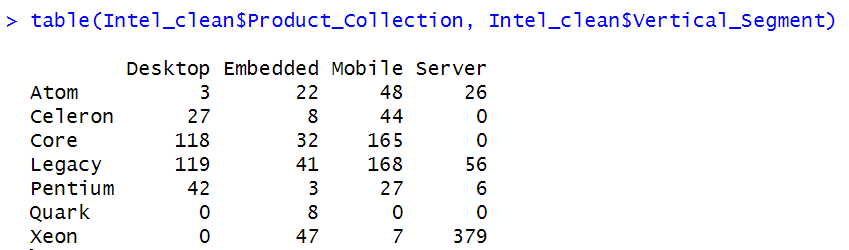
\includegraphics[width=14cm]{img/1.png}
  \caption{Data Partition based on \texttt{Product\_Collection} and \texttt{Vertical\_Segment}}
\end{figure}

\subsection{Hypotheses Testing}

\begin{lstlisting}[language=R]

  \end{lstlisting}

% Rút gọn tên biến, chuyển các yếu tố định tính về nhân tố thống kê (factor).
% \begin{figure}[h!]
%  \begin{left}
%   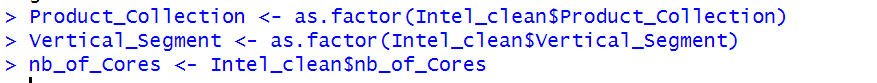
\includegraphics[width=12cm]{img/2.png}
%  \end{left}
% \end{figure}
% \\
% Kiểm tra dữ liệu nb\_of\_Cores có theo phân phối chuẩn hay không bằng Shapiro-Wilk test. \\
% Thư viện: \texttt{library(nortest)} \\
% Lệnh: \texttt{shapiro.test()} \\
% Giả thuyết:

% $H_0$: biến \texttt{nb\_of\_Cores} tuân theo phân phối chuẩn.

% $H_1$: biến \texttt{nb\_of\_Cores} không tuân theo phân phối chuẩn.
% \begin{figure}[h!]
%  \begin{left}
%   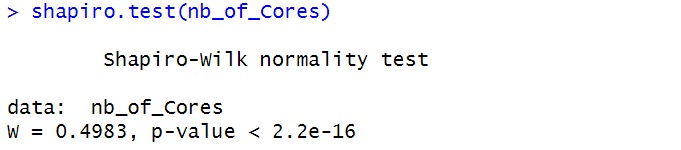
\includegraphics[width=12cm]{3.png}
%  \end{left}
% \end{figure} \\
% Nhận xét: p-value = $2.2 e-16 < 0.05$, ta bác bỏ giả thuyết $H_0$ hay nói cách khác biến \texttt{nb\_of\_Cores} không tuân theo phân phối chuẩn. \\
% Vẽ biểu đồ Q-Q Plot để có cái nhìn trực quan hơn về tính phân phối chuẩn của biến \texttt{nb\_of\_Cores}. \\
% Thư viện: \texttt{library(ggpubr)} \\
% Lệnh: \texttt{ggqqplot()}
% \begin{figure}[h!]
%  \begin{left}
%   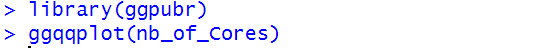
\includegraphics[width=12cm]{4.png}
%  \end{left}
% \end{figure} \\
% Kết quả:
% \begin{figure}[h!]
%  \begin{left}
%   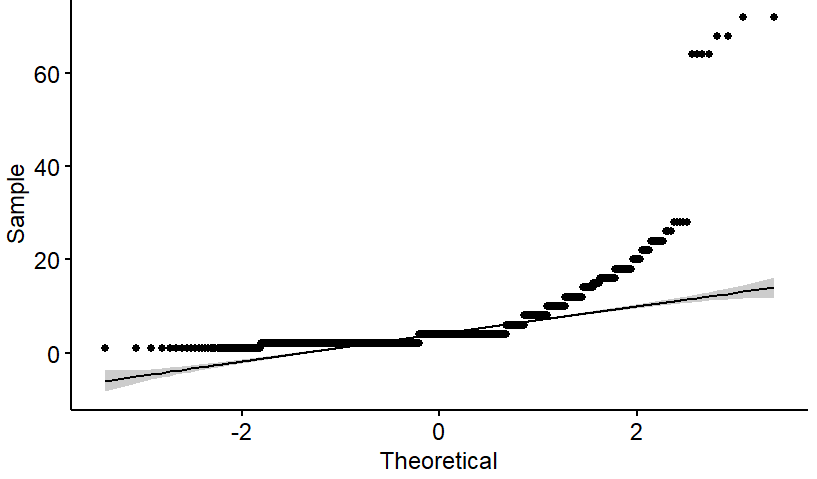
\includegraphics[width=15cm]{5.png}
%  \end{left}
% \end{figure} \\ \\ \\ \\ \\ \\
% Nhận xét: Biểu đồ QQ-plot cho ta thấy những giá trị quan sát đa phần không nằm trên đường thẳng kì vọng của phân phối chuẩn, do đó biến \texttt{nb\_of\_Cores} không tuân theo phân phối chuẩn. \\
% Kiểm định tính đồng nhất của phương sai dữ liệu bằng Levene's test.\\
% Thư viện: \texttt{library(car)}\\
% Lệnh: \texttt{leveneTest()}\\
% Giả thuyết:

% $H_0$: phương sai của các nhóm dữ liệu bằng nhau.

% $H_1$: tồn tại hai nhóm dữ liệu có phương sai khác nhau.
% \begin{figure}[h!]
%  \begin{left}
%   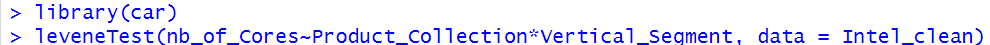
\includegraphics[width=15cm]{6.png}
%  \end{left}
% \end{figure} \\
% Kết quả:
% \begin{figure}[h!]
%  \begin{left}
%   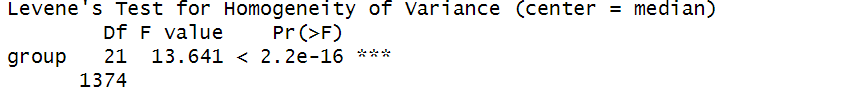
\includegraphics[width=12cm]{7.png}
%  \end{left}
% \end{figure}

% Nhận xét: $p\text{-value} < 2.2 e-16$ là rất nhỏ, nhỏ hơn 0.05, ta bác bỏ giả thuyết $H_0$ hay nói cách khác các nhóm dữ liệu có phương sai không đồng nhất.

% Kết luận: do dữ liệu \texttt{nb\_of\_Cores} không tuân theo phân phối chuẩn và các nhóm dữ liệu không có phương sai đồng nhất nên không thỏa mãn điều kiện bài toán Anova hai nhân tố. Nhưng do đây là một mẫu lớn nên ta có thể bỏ qua vi phạm này.

% Thực hiện phân tích Anova hai nhân tố:

% Mục đích: Kiểm tra sự ảnh hưởng của hai nhân tố \texttt{Product\_Collection} và \texttt{Vertical\_Segment} đối với \texttt{nb\_of\_Cores}.

% Do đây là một mẫu lớn nên dù mẫu đã vi phạm các giả định về phân phối chuẩn và phương sai đồng nhất thì phương pháp ANOVA hai nhân tố vẫn có thể áp dụng được. Tuy nhiên kết quả chỉ mang tính chất tham khảo, nếu muốn có kết quả chính xác hơn thì ta có thể sử dụng những phương pháp khác.

% Ta sẽ kiểm định các nhóm có số lượng mẫu lớn (>30).

% Chọn dữ liệu đầu vào:
% \begin{itemize}
%  \item \texttt{Product\_Collection}: Core, Legacy.
%  \item \texttt{Vertical\_Segment}: Desktop, Embedded, Mobile.
% \end{itemize}
% \newpage
% \begin{figure}[h!]
%  \begin{left}
%   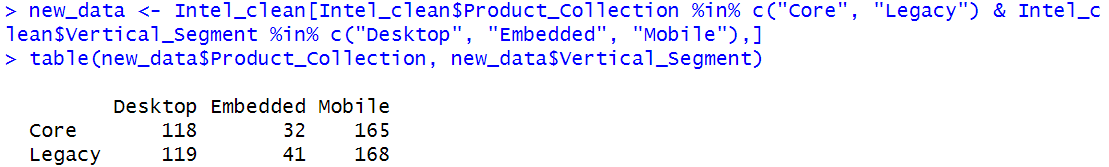
\includegraphics[width=15cm]{8.png}
%  \end{left}
% \end{figure} \\ \\ \\ \\ \\
% Rút gọn tên biến, chuyển các yếu tố định tính về nhân tố thống kê (factor).
% \begin{figure}[h!]
%  \begin{left}
%   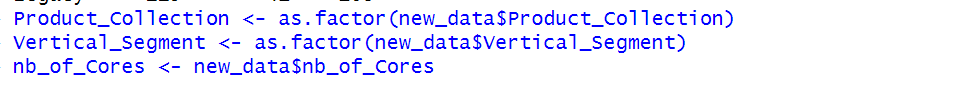
\includegraphics[width=15cm]{9.png}
%  \end{left}
% \end{figure} \\
% Dùng lệnh aov() để phân tích Anova rồi lưu kết quả vào av, để hiển thị kết quả ta dùng lệnh summary(av). \\
% Kết quả:
% \begin{figure}[h!]
%  \begin{left}
%   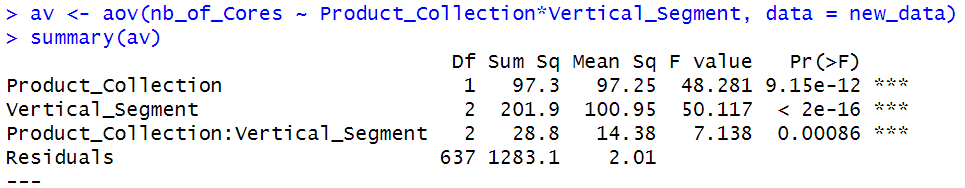
\includegraphics[width=12cm]{10.png}
%  \end{left}
% \end{figure} \\
% Trong kết quả trên, có các cột: Df (degrees of freedom) là bậc tự do; Sum Sq là tổng bình phương (sum of squares), Mean Sq là trung bình bình phương (mean square); F value là giá trị F; và Pr(>F) là trị số P liên quan đến kiểm định F. \\
% \textbf{Nhận xét:} Qua trung bình bình phương (Mean sq), chúng ta thấy ảnh hưởng của Product\_Collection và Vertical\_Segment có vẻ là như nhau, và cả hai ảnh hưởng đều có ý
% nghĩa thống kê, vì trị số p rất thấp cho hai yếu tố, cụ thể:\\
% \textbf{Đối với Product\_Collection:} \\
% Giả thuyết:

% $H_0$: số lõi CPU trung bình ở hai loại sản phẩm Core và Legacy là giống nhau.

% $H_1$: số lõi CPU trung bình ở hai loại sản phẩm Core và Legacy là khác nhau.
% \\
% Nhận xét: vì $p\text{-value} = 0.15 e-12 < 0.05$ nên ta bác bỏ giả thuyết $H_0$.\\
% \textbf{Đối với Vertical\_Segment:}\\
% Giả thuyết:

% $H_0$: số lõi CPU trung bình ở các phân khúc ứng dụng Desktop, Embedded, Mobile là giống nhau.

% $H_1$: có ít nhất hai phân khúc có số lõi CPU trung bình khác nhau.\\
% Nhận xét: vì $p\text{-value} < 2 e-16$ là rất nhỏ so với 0.05 nên ta bác bỏ giả thuyết $H_0$.\\
% \textbf{Kết luận:} số lõi CPU trung bình là khác nhau đối với các dòng sản phẩm (\texttt{Product\_Collection}) và phân khúc ứng dụng (\texttt{Vertical\_Segment}) khác nhau, nên số lõi CPU trung bình phụ thuộc vào dòng sản phẩm và phân khúc ứng dụng.
